% CS 5788 Final Project Report
% Use the page-numbered version of the CVPR 2026 template.

\documentclass[10pt,twocolumn,letterpaper]{article}

% \usepackage{cvpr}              % camera-ready
% \usepackage[review]{cvpr}      % review (line numbers)
\usepackage[pagenumbers]{cvpr}   % page-numbered (per CS5788 instructions)

% Inline annotation helpers
\newcommand{\red}[1]{{\color{red}#1}}
\newcommand{\todo}[1]{{\color{red}#1}}
\newcommand{\TODO}[1]{\textbf{\color{red}[TODO: #1]}}

% disable for camera ready by uncommenting:
% \renewcommand{\TODO}[1]{}
% \renewcommand{\todo}[1]{#1}

% Useful packages
\usepackage{graphicx}
\usepackage{amsmath}
\usepackage{amssymb}
\usepackage{booktabs}
\usepackage{microtype}

% Math operators
\DeclareMathOperator*{\argmin}{arg\,min}
\DeclareMathOperator*{\argmax}{arg\,max}


\definecolor{cvprblue}{rgb}{0.21,0.49,0.74}
\usepackage[pagebackref,breaklinks,colorlinks,allcolors=cvprblue]{hyperref}
\usepackage{tikz}
\usetikzlibrary{arrows.meta, positioning, shapes.geometric}

\def\paperID{CS5788} % course-internal ID
\def\confName{CS 5788}
\def\confYear{2026}

\title{Three Ways to Rewrite a Photograph: \\ Object Replacement, Relocation, and Style Transfer with Stable Diffusion}

\author{Stefan Arni Arnarsson \\
Cornell Tech \\
{\tt\small sa2467@cornell.edu}
\and
Aryaan Verma \\
Cornell Tech \\
{\tt\small av629@cornell.edu}
\and
Chien-Wei Wang \\
Cornell Tech \\
{\tt\small cw2245@cornell.edu}
}


\begin{document}
\maketitle

%-----------------------------------------------------------------------
%  ABSTRACT
%-----------------------------------------------------------------------
\begin{abstract}
We build three text and mask driven editing pipelines on Stable Diffusion, exposed through one Gradio app. \emph{Object replacement} swaps an object in a real photograph using SD 1.5 with null-text inversion, a novel per-token attention swap schedule, and a pixel-space composite over an attention-derived mask. \emph{Object relocation} moves an object within the same frame using DDPM noise-prior shifting on SD 2.1 plus an SD 2.1 inpainting cleanup of the vacated source. \emph{Style transfer} repaints the photo via per-style LoRA adapters trained on WikiArt and blended at inference. For replacement, the pixel composite cuts background LPIPS by 98\% across 20 BLIP-captioned COCO photos (from $0.38$ to $0.008$) and by 92\% on the cat$\to$dog case study, where CLIP directional similarity reaches 0.55. The schedule-shape effect itself is within image-to-image variance, indicating the mask plus composite is the dominant operational lever. For relocation, our pipeline lowers VGG perceptual distance at the target by 6.1\% over an SDEdit-only baseline at matched harmonization, isolating the noise shift as the source of the texture-preservation gain. For style, all five WikiArt LoRA adapters (Van Gogh, Seurat, Monet, Ukiyo-e, Picasso) train to convergence at 500 steps and blend cleanly at inference.
\end{abstract}

%-----------------------------------------------------------------------
%  1.  INTRODUCTION
%-----------------------------------------------------------------------
\section{Introduction}
\label{sec:intro}

Most people treat a photograph as fixed once it is taken. Recent generative tools (Adobe Generative Fill, Photoshop Content-Aware, Midjourney) have begun to change that, but they ship as black boxes with proprietary models and large-scale fine-tuning. We wanted to see how far the opposite recipe gets us: off-the-shelf Stable Diffusion checkpoints~\cite{rombach2022sd}, classical attention-control techniques from the recent literature, and only lightweight per-style LoRA adapters where fine-tuning is unavoidable. Our project covers three complementary edits on one input photograph: \textbf{object replacement} swaps one object for another from text prompts, \textbf{object relocation} moves an object to a user painted target location and fills the vacated source, and \textbf{style transfer} repaints the photo using LoRA-adapter styles trained on WikiArt. The three are independent pipelines sharing a single Gradio interface so one photo can cascade through all three.

\paragraph{Related work.}
Prompt-to-Prompt~\cite{hertz2022p2p} introduced cross-attention swapping for text-prompted edits: pasting the source prompt's attention maps into the target's UNet for the first $\tau T$ steps preserves spatial structure while semantic content swaps. Null-text inversion~\cite{mokady2022nullinv} extends it to real photos by inverting with DDIM~\cite{song2021ddim} and optimizing per-timestep null embeddings so CFG sampling tracks the inversion. Blended Latent Diffusion~\cite{avrahami2022blended} blends a noised source into the denoising trajectory for mask-localized inpainting, which we use for size-mismatch edits. LoRA~\cite{hu2021lora} provides parameter-efficient adapters trainable on small style sets and blendable at inference. Imagic and InstructPix2Pix take a different route by fine-tuning per image or training a custom instruction-following backbone, both of which we avoid.

\paragraph{Our contributions.}
\begin{enumerate}
    \itemsep0em
    \item \textbf{(Replacement)} A per-token, per-timestep attention swap schedule (five shape primitives, three token roles) paired with a pixel-space composite that keeps non-edited pixels identical to the source, a three-region extension for size-mismatch edits, and BLIP-captioned source prompts that double as mislabeled-COCO-category catchers (\S\ref{sec:replace}).
    \item \textbf{(Relocation)} A DDPM-inversion plus per-step noise-prior shift pipeline for texture-preserving object relocation, with a Gaussian-fill pixel composite as the SDEdit start, RePaint-style background and target locks during harmonization, and a separate SD 2.1 inpainting cleanup of the vacated source region (\S\ref{sec:relocate}).
    \item \textbf{(Style)} Per-style LoRA adapters (rank 8, alpha 16, $\sim$6.1\,MB each) trained on 100 WikiArt samples per style, blended at inference via diffusers' \texttt{set\_adapters} with weights normalized to one (\S\ref{sec:style}).
    \item \textbf{(Joint)} A unified Gradio platform that wires all three editing pipelines into one interface with cascading hand-offs and lazy per-tab model loading (\S\ref{sec:platform}).
\end{enumerate}

%-----------------------------------------------------------------------
%  2.  METHOD
%-----------------------------------------------------------------------
\section{Method}
\label{sec:method}

All three modules run at $512 \times 512$. Replacement loads SD 1.5 components individually (UNet, VAE, CLIP, DDIM) so the cross-attention controller can hook every denoising step. Relocation loads SD 2.1 components individually with the DDPM scheduler (the noise shift needs transition noises) and uses diffusers' packaged \texttt{StableDiffusionInpaintPipeline} for the source-region cleanup. Style uses \texttt{StableDiffusionImg2ImgPipeline} with SD 1.5 plus LoRA weights via \texttt{set\_adapters}.

\begin{figure}[t]
    \centering
    \begin{tikzpicture}[
        node distance=2.5mm and 3mm,
        font=\scriptsize,
        every node/.style={align=center},
        box/.style={draw, rounded corners=1.5pt, minimum width=14mm, minimum height=5mm, inner sep=1pt},
        op/.style={box, fill=cvprblue!8},
        out/.style={box, fill=black!4},
        arrow/.style={-{Latex[length=1.5mm]}, thick}
    ]
    \node[out] (img) {input \\ photo};
    \node[op, right=of img] (inv) {null-text \\ inversion};
    \node[op, right=of inv] (samp) {4-way \\ sample};
    \node[op, right=of samp] (mask) {scout \\ + mask};
    \node[op, below=of samp] (sched) {schedule \\ controller};
    \node[op, below=of mask] (comp) {pixel \\ composite};
    \node[out, below=of inv] (final) {edited \\ photo};
    \draw[arrow] (img) -- (inv);
    \draw[arrow] (inv) -- (samp);
    \draw[arrow] (samp) -- (mask);
    \draw[arrow] (sched) -- (samp);
    \draw[arrow] (mask) -- (comp);
    \draw[arrow] (comp) -- (final);
    \draw[arrow] (img.south) -- ++(0,-9mm) -| (comp.south);
    \end{tikzpicture}
    \caption{\textbf{Replacement pipeline.} Null-text inversion, 4-way batched sampling under a schedule controller that blends cross-attention by token column, and a final pixel composite under a scout-derived mask.}
    \label{fig:teaser}
\end{figure}

\subsection{Object Replacement}
\label{sec:replace}

\paragraph{Per-token attention swap schedule.}
Vanilla Prompt-to-Prompt~\cite{hertz2022p2p} exposes one knob $\tau \in [0, 1]$. Cross-attention maps from the source prompt are pasted into the target's UNet for steps $t/T < \tau$, then dropped. We generalize this with a soft swap whose weight depends on a token role and the normalized timestep $t_{\text{frac}} \in [0, 1]$:
\begin{equation}
    A^{\text{tgt}}_{t, \ell, j} \;\leftarrow\; w \cdot A^{\text{src}}_{t, \ell, j} + (1 - w) \cdot A^{\text{tgt}}_{t, \ell, j}, \quad w = w(t_{\text{frac}}, \, \text{role}(j))
\label{eq:blend}
\end{equation}
where $A^{(\cdot)}_{t, \ell, j}$ is the cross-attention map at timestep $t$, layer $\ell$, prompt-token column $j$. Each position is classified by comparing source and target CLIP token IDs. Matching positions are \emph{preserved}, differing positions are \emph{replaced}, and special tokens are \emph{context}. A \texttt{ScheduleSet} bundles three callables, one per role, picking from five shapes: \texttt{Constant}, \texttt{LinearDecay}, \texttt{Cosine}, \texttt{Step}, \texttt{Piecewise}. Our P2P-style baseline uses preserved \texttt{Step}$(\tau, 1, 0)$ and replaced \texttt{Constant}$(0)$. Since early timesteps fix layout~\cite{hertz2022p2p}, we expect structural edits (cat$\to$dog) to favor a fast-decaying replaced-token weight, and geometric edits (apple$\to$banana) to favor a slower decay so the target prompt can establish the new layout. We swap diffusers' \texttt{AttnProcessor2\_0} for a custom processor that routes the post-softmax probabilities through our \texttt{ScheduleController}, and batch the UNet input as \texttt{[null$_t$, cond$_{\text{src}}$, null$_t$, cond$_{\text{tgt}}$]} so both paths share a single forward call.

\paragraph{Mask and pixel composite.}
We derive a localization mask by averaging cross-attention at the source-token columns over mid-timesteps ($t_{\text{frac}} \in [0.3, 0.7]$) and over UNet layers at the $16{\times}16$ and $32{\times}32$ resolutions. The averaged $64{\times}64$ map is thresholded at the 80th percentile, dilated 2 pixels, and softly blurred. Latent-space blending alone leaves a small footprint on background pixels because of VAE round-trip noise. To make the background bit-exact we add a final pixel-space composite $I^{\text{out}} = M \cdot I^{\text{edit}} + (1 - M) \cdot I^{\text{src}}$, where $M$ is the upsampled mask. We center-crop to a square before SD touches the image and paste the result back into the original frame at full resolution, so any input aspect ratio is preserved.

\paragraph{Three-region composite and BLIP-captioned source prompts.}
When the target object is much smaller than the source (e.g.\ dog$\to$mouse), the source-shape mask leaves an awkward gap. The \texttt{ScheduleController} optionally captures target-side conditional attention to derive a second mask $M^{\text{tgt}}$ for where the target actually renders. The leftover region $M^{\text{diff}} = M^{\text{src}} \setminus M^{\text{tgt}}$ is filled by a separate blended-diffusion~\cite{avrahami2022blended} pass driven by a background-only prompt. The final composite has three regions: original pixels outside $M^{\text{src}}$, the edit inside $M^{\text{tgt}}$, and the inpainted background inside $M^{\text{diff}}$. Real photographs need one further trick. A bare prompt like ``a photograph of a cat'' over a busy scene makes null-text inversion drift, so we caption each input with BLIP~\cite{li2022blip} and substitute the swap word for the target prompt. As a side effect, if the source word never appears in the BLIP caption, the COCO category label is probably wrong for that image and we drop it from the ablation set.

\subsection{Object Relocation}
\label{sec:relocate}

\paragraph{Initial composite and DDPM inversion.}
We translate the source-mask object pixels by the centroid offset $\Delta$ and paste them at the target location. The vacated hole is filled by weighted Gaussian propagation (background pixels and a binary weight mask blurred together at radius $r = \max(\text{box\_h}, \text{box\_w})$, then divided channel-wise) which gives the SDEdit pass a coherent starting image rather than a hard-edged void. We then DDPM-invert at $T = 50$ steps, storing both the marginal noise $\epsilon_t$~\cite{ho2020ddpm} and the transition noise $z_t$ from the posterior $q(x_{t-1} \mid x_t, x_0)$. DDIM inversion~\cite{song2021ddim} would store only latents, which exposes $\epsilon_t$ pointwise but not the stochastic increment our shift step needs to translate across the frame.

\paragraph{Source-to-target noise shift.}
Building on InstructUDrag's~\cite{yu2025instructudrag} DDPM noise-prior shift, we adapt the idea to operate on the stored noise $\epsilon_t$ with Gaussian-feathered source and target masks and an affine-grid-based shift:
\begin{equation}
    \epsilon^{\text{shift}}_t \;=\; \epsilon_t \odot (1 - M^{\text{src}}_{\text{soft}})(1 - M^{\text{tgt}}_{\text{soft}}) \;+\; \mathcal{W}_{\Delta}\!\bigl(\epsilon_t \odot M^{\text{src}}_{\text{soft}}\bigr),
\label{eq:shift}
\end{equation}
where $M^{(\cdot)}_{\text{soft}}$ are Gaussian-feathered ($\sigma = 2$) latent-resolution masks and $\mathcal{W}_{\Delta}$ is an affine sampler translating content by the centroid offset $\Delta$. Zeroing the noise inside both regions before adding the shifted source noise prevents superposition. The shift is applied to both $\epsilon_t$ and $z_t$ so the reverse trajectory remains consistent. The centroid-only shift presupposes source and target masks of similar shape and scale, a limitation we revisit in \S\ref{sec:exp:relocate}.

\paragraph{Harmonization, cleanup, and final composite.}
An SDEdit pass~\cite{meng2022sdedit} starts from the pre-fill composite at \texttt{sdedit\_strength}~$= 0.7$ and denoises back to $t = 0$ along the shifted DDPM trajectory. Two RePaint-style~\cite{lugmayr2022repaint} locks run during the denoise: a \emph{background lock} copies the inverted background latent over the predicted latent at every step so pixels outside both masks track the original, and a \emph{target lock} copies the composite-driven latent over the target region for the first quarter of active steps to anchor the moved object. We then fill the vacated source region with an SD 2.1 inpainting pass~\cite{rombach2022sd} reading the Gaussian-filled composite (an empty positive prompt with a category-specific negative prompt biases the model toward background texture). The final image is a four-way pixel-space blend: the target region mixes the SDEdit output with a centroid-aligned paste of the original source pixels ($\alpha = 0.75$ on the paste, identical in both ablation arms, so the noise shift's effect is on the SDEdit-output share), the source region (excluding target overlap) uses the inpainting output, and the rest is the original photograph at full resolution. The ablation in \S\ref{sec:exp:relocate} flips \texttt{use\_noise\_shift = False}.

\subsection{Style Transfer}
\label{sec:style}

\paragraph{Per-style LoRA training.}
We support five painterly styles: Van Gogh, Seurat, Monet, Ukiyo-e, and Picasso. Each training set is built by streaming \texttt{huggan/wikiart} (~81K images) and filtering on the artist class label, except Ukiyo-e which filters on the style class label since it is a movement rather than a single artist. We sample 100 images per style at $512 \times 512$. All five adapters share an identical LoRA configuration injected into SD 1.5's UNet cross-attention layers: rank 8, alpha 16, targeting \texttt{to\_q}, \texttt{to\_k}, \texttt{to\_v}, \texttt{to\_out.0}. Trained for 500 steps per style with AdamW at learning rate $10^{-4}$ on Apple Silicon (MPS, fp32). All other experiments run on the A100. Each image uses the fixed caption \texttt{a painting in the style of <artist>}.

\paragraph{Multi-style blending at inference.}
The user picks up to three styles with weights $w_i \in [0, 1]$. We normalize the weights to sum to one and call \texttt{set\_adapters}, which activates the chosen adapters simultaneously in a single forward pass. The trigger phrases concatenate, so a 50/50 Van Gogh and Monet mix becomes \texttt{a painting in the style of van gogh, a painting in the style of claude monet}. The blend runs through \texttt{StableDiffusionImg2ImgPipeline} at user-controlled \texttt{strength} and \texttt{guidance\_scale}.

\subsection{Unified Platform}
\label{sec:platform}

The three modules share a single Gradio app. Each loads its SD checkpoints lazily on first tab use, and all three weight sets fit comfortably on one A100. The interface offers cascading hand-offs: the replacement tab's output feeds the relocation tab as a new source, and from there into the style tab, so one uploaded photograph can carry through replace, relocate, then restyle in a single session.

%-----------------------------------------------------------------------
%  3.  EXPERIMENTS
%-----------------------------------------------------------------------
\section{Experiments}
\label{sec:experiments}

\subsection{Setup}
\label{sec:setup}

We run on an NVIDIA A100 at $512 \times 512$, 50 DDIM steps, CFG 7.5 unless noted. Replacement and style use SD 1.5 (\texttt{stable-diffusion-v1-5} community mirror); relocation uses SD 2.1 plus the SD 2.1 inpainting checkpoint. For real photographs we use a 20-image subset of COCO val2017~\cite{lin2014coco} auto-curated to images where one object covers at least 10\% of the frame, across 10 swap pairs (cat, dog, horse, zebra, apple, banana, cup, bowl, pizza). Source prompts are auto-captioned with BLIP-base~\cite{li2022blip}. Metrics: reconstruction LPIPS~\cite{zhang2018lpips}, CLIP directional similarity~\cite{gal2022stylegannada}, and background LPIPS (computed outside the attention mask).

\subsection{Object Replacement Results}
\label{sec:exp:repl}

\paragraph{Reconstruction and case-study schedule ablation.}
On a generated cat-on-couch image, 50-step null-text inversion at 10 inner Adam steps reaches reconstruction LPIPS of 0.017, under the 0.05 proposal target. Real COCO photos average 0.06-0.10, matching~\cite{mokady2022nullinv}. On the cat$\to$dog case study (Table~\ref{tab:schedules}), linear decay on the replaced token slightly beats vanilla P2P and constant-0.5 (slow blend) is worst, consistent with our prediction (\S\ref{sec:replace}) that fast decay benefits structural edits. As reported below, this per-image win does not generalize.

\begin{table}[t]
    \centering
    \small
    \begin{tabular}{lcc}
        \toprule
        \textbf{Schedule (replaced token)} & \textbf{CLIP-dir $\uparrow$} & \textbf{full LPIPS $\downarrow$} \\
        \midrule
        Vanilla P2P (Step($0.8$, $1$, $0$)) & $0.5312$ & $0.4217$ \\
        Linear decay (\textbf{ours}) & $\mathbf{0.5398}$ & $0.3643$ \\
        Cosine decay & $0.5360$ & $0.3628$ \\
        Constant $0.5$ (slow blend) & $0.5077$ & $0.3915$ \\
        Piecewise (3-knot) & $0.5387$ & $0.3656$ \\
        \bottomrule
    \end{tabular}
    \caption{\textbf{Schedule ablation (case study).} cat$\to$dog on the generated cat-on-couch image. Preserved tokens use \texttt{Constant}$(1.0)$. CLIP-dir is computed against ``a photograph of a cat / dog sitting on a couch''. Linear decay edges out vanilla P2P here, but the effect collapses into image-to-image variance on the 20-photo set.}
    \label{tab:schedules}
\end{table}

\paragraph{Background preservation and 20-photo generalization.}
On the cat$\to$dog edit, switching from no-mask baseline (CLIP-dir 0.531, bg-LPIPS 0.242) to attention-mask plus pixel composite gives CLIP-dir 0.550 and bg-LPIPS 0.019, a 92\% reduction in background drift. Across the broader 20-photo set the same recipe reduces bg-LPIPS from $0.38 \pm 0.16$ to $0.008 \pm 0.011$ averaged over all schedules, a 98\% reduction. Mean CLIP-dir falls in $[0.20, 0.21]$ across all five shapes with per-image std $\sim 0.14$, so the per-image schedule win does not generalize. The dominant operational lever is the mask plus pixel composite, not the schedule shape.

\begin{figure}[t]
    \centering
    \IfFileExists{figures/qualitative.pdf}{%
        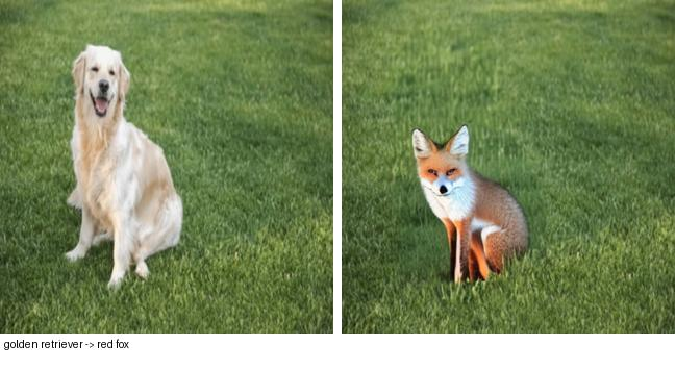
\includegraphics[width=0.9\linewidth]{figures/qualitative.pdf}%
    }{%
        \fbox{\rule{0pt}{1.6in}\rule{0.9\linewidth}{0pt}}%
    }
    \caption{\textbf{Qualitative replacement result.} Golden retriever $\to$ red fox using \texttt{LinearDecay}$(1{\to}0)$ on the replaced token, attention mask, and pixel composite. Outside the soft mask falloff, pixels are identical to the source by construction.}
    \label{fig:qual}
\end{figure}

\paragraph{Failure modes.}
\label{sec:exp:fails}
Beyond the BLIP-caught COCO label noise (\S\ref{sec:replace}), two failure modes recur on real photos. First, VAE round-trip blur: SD 1.5's encoder-decoder noticeably blurs fine high-entropy textures even before inversion runs, the dominant source of reconstruction error. Second, in-mask shape mismatch: a much smaller target gets stretched to fill the source silhouette, which the three-region composite addresses.

\subsection{Object Relocation Results}
\label{sec:exp:relocate}

\paragraph{Quantitative (case study, $n{=}1$).}
Table~\ref{tab:relocate} compares our DDPM noise-shift pipeline against the SDEdit baseline on a single synthetic orange-ball move, holding everything except the per-step spatial shift fixed. The noise-shift pass lowers perceptual distance at the target by 6.1\% ($1.570$ vs.\ $1.672$). We report this as a case study, not a benchmark. CLIP score is essentially tied (0.343 vs.\ 0.344) and background PSNR/SSIM are identical to two decimals (53.5\,dB / 0.998) since both arms apply the same background lock and pixel composite by construction.

\begin{table}[t]
    \centering
    \small
    \begin{tabular}{lcc}
        \toprule
        \textbf{Variant} & \textbf{Perc.\ dist $\downarrow$} & \textbf{CLIP $\uparrow$} \\
        \midrule
        SDEdit baseline & $1.672$ & $0.344$ \\
        + noise shift (\textbf{ours}) & $\mathbf{1.570}$ & $0.343$ \\
        \bottomrule
    \end{tabular}
    \caption{\textbf{Relocation case study.} Single synthetic orange-ball move. Perceptual distance is VGG \texttt{relu3\_3}~\cite{zhang2018lpips} between source and target crops at $256{\times}256$ (lower is better). CLIP score~\cite{radford2021clip}: image-text similarity vs.\ the move prompt.}
    \label{tab:relocate}
\end{table}

\paragraph{Qualitative.}
Figure~\ref{fig:relocate-qual} shows the orange-ball move. The texture transplant carries the original gradient and speckle from the source ball into the target, while the SDEdit baseline preserves the silhouette but reverts the inside texture to the model prior. The pipeline presupposes visually similar source and target backgrounds and masks of similar shape and scale, since the centroid-only shift cannot stretch or shrink. Two failure modes follow: scale mismatch leaves the moved object at the wrong size, and the inpainting cleanup occasionally hallucinates small objects on visually busy backgrounds.

\begin{figure}[t]
    \centering
    \IfFileExists{figures/relocate_qualitative.pdf}{%
        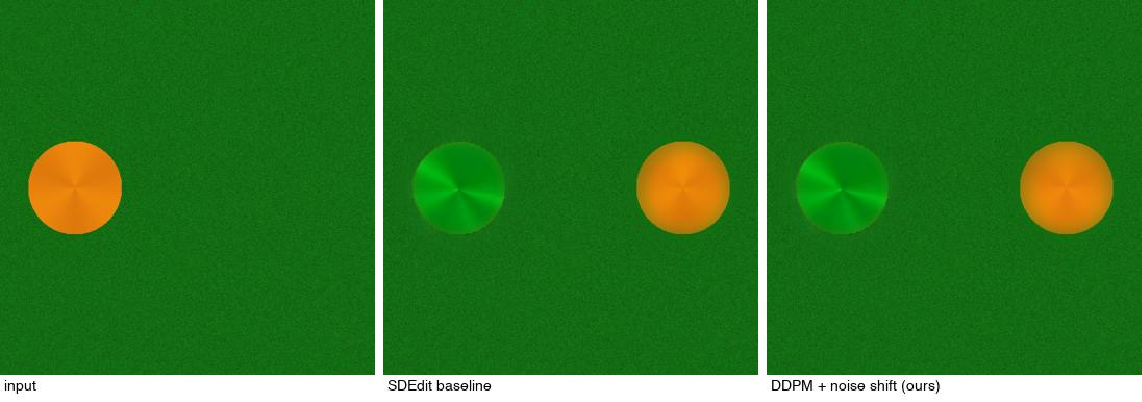
\includegraphics[width=0.9\linewidth]{figures/relocate_qualitative.pdf}%
    }{%
        \fbox{\rule{0pt}{1.4in}\rule{0.9\linewidth}{0pt}}%
    }
    \caption{\textbf{Qualitative relocation.} Orange-ball move from left to right: input, SDEdit baseline (no shift), and ours.}
    \label{fig:relocate-qual}
\end{figure}

\subsection{Style Transfer Results}
\label{sec:exp:style}

All five styles trained to completion at 500 steps with final smoothed losses around 0.1. Single-style runs match their training corpus qualitatively (impasto for Van Gogh, pointillist dots for Seurat, etc.), and multi-style blends interpolate coherently (a 50/50 Van Gogh and Monet mix applies impressionist light diffusion with Van Gogh's palette). We did not compute formal Gram-matrix or LPIPS metrics for this submission.

%-----------------------------------------------------------------------
%  4.  CONCLUSION
%-----------------------------------------------------------------------
\section{Conclusion}
\label{sec:conclusion}

We built three Stable Diffusion editing pipelines tied together by one Gradio cascade. \textbf{Replacement}'s mask plus pixel composite reduces bg-LPIPS by 98\% across 20 real photos, with the schedule shape itself within image-to-image variance. \textbf{Relocation}'s per-step source-to-target noise shift (Eq.~\ref{eq:shift}) lowers target perceptual distance by 6.1\% over a matched SDEdit baseline. \textbf{Style transfer}'s five LoRA adapters train to convergence and blend cleanly at inference. Limitations: SD 1.5's VAE blur on fine textures, the centroid-only shift's shape-and-scale assumption, and no formal style-strength metrics.

%-----------------------------------------------------------------------
%  REFERENCES
%-----------------------------------------------------------------------
{
    \small
    \bibliographystyle{ieeenat_fullname}
    \bibliography{main}
}

\end{document}
